\documentclass[10pt,aspectratio=169]{beamer}

% Theme selection
\usetheme{metropolis}
\usecolortheme{default}

% Packages
\usepackage[utf8]{inputenc}
\usepackage{graphicx}
\usepackage{booktabs}
\usepackage{listings}
\usepackage{xcolor}
\usepackage{tikz}
\usetikzlibrary{shapes.geometric, arrows, positioning}

% Code styling
\definecolor{codegreen}{rgb}{0,0.6,0}
\definecolor{codegray}{rgb}{0.5,0.5,0.5}
\definecolor{codeblue}{rgb}{0.1,0.1,0.8}
\lstset{
    language=Go,
    basicstyle=\tiny\ttfamily,
    keywordstyle=\color{codeblue},
    commentstyle=\color{codegray},
    stringstyle=\color{orange},
    breaklines=true,
    showstringspaces=false,
    frame=single,
    rulecolor=\color{lightgray}
}

% Metadata
\title{MapReduce on Kubernetes}
\subtitle{A Deep Dive into Distributed Parallel Computing with Go}
\author{Advanced Distributed Systems Group}
\date{\today}

\begin{document}

% --- Title Page ---
\maketitle

% --- Table of Contents ---
\begin{frame}{Agenda}
    \setbeamertemplate{section in toc}[sections numbered]
    \tableofcontents[hideallsubsections]
\end{frame}

% ==========================================
% SECTION 1: INTRODUCTION & VISION
% ==========================================
\section{Introduction \& Project Vision}

\begin{frame}{The Evolution of Data Processing}
    \begin{itemize}
        \item \textbf{Legacy:} Static clusters, manual resource allocation, "noisy neighbor" issues.
        \item \textbf{Modern:} Cloud-native, containerized, elastic scaling.
        \item \textbf{The Goal:} Re-implementing the classic MapReduce paradigm (Dean \& Ghemawat) using 2026-era cloud technologies.
        \item \textbf{Primary Objective:} Zero-friction job submission with industrial-grade reliability.
    \end{itemize}
\end{frame}

\begin{frame}{Why Go + Kubernetes?}
    \begin{columns}
        \begin{column}{0.5\textwidth}
            \textbf{Go (The Language):}
            \begin{itemize}
                \item Static binaries (easy containerization).
                \item High-performance concurrency (Goroutines).
                \item Native plugin support (via \texttt{go-plugin}).
            \end{itemize}
        \end{column}
        \begin{column}{0.5\textwidth}
            \textbf{Kubernetes (The Platform):}
            \begin{itemize}
                \item Orchestration at scale.
                \item Ephemeral \texttt{batch/v1} Jobs.
                \item Native networking and discovery.
            \end{itemize}
        \end{column}
    \end{columns}
\end{frame}

% ==========================================
% SECTION 2: ARCHITECTURE DEEP DIVE
% ==========================================
\section{Architecture Deep Dive}

\begin{frame}{Service Orchestration}
    \centering
    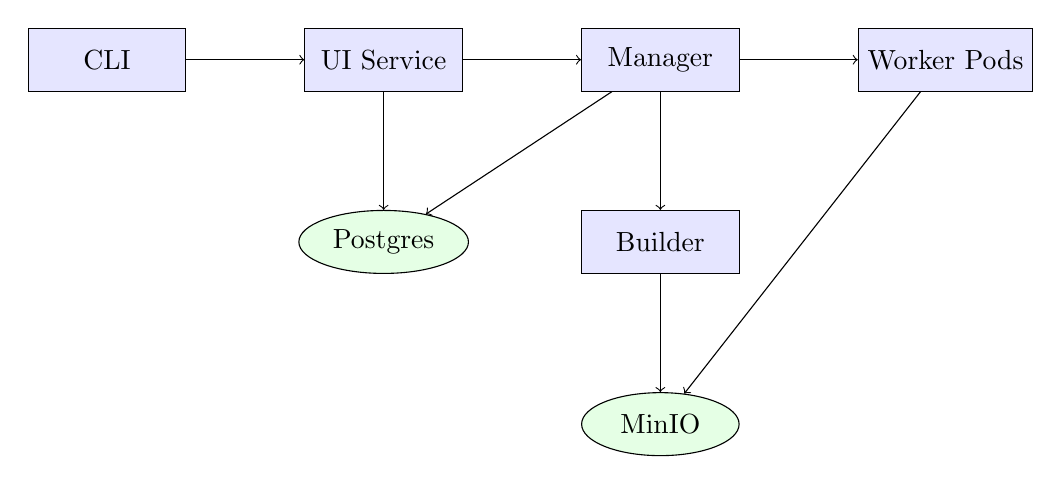
\begin{tikzpicture}[node distance=1.5cm, auto]
        \tikzstyle{service} = [rectangle, minimum width=2cm, minimum height=0.8cm, text centered, draw=black, fill=blue!10]
        \tikzstyle{infra} = [ellipse, minimum width=2cm, minimum height=0.8cm, text centered, draw=black, fill=green!10]
        
        \node (cli) [service] {CLI};
        \node (ui) [service, right=of cli] {UI Service};
        \node (manager) [service, right=of ui] {Manager};
        \node (builder) [service, below=of manager] {Builder};
        \node (worker) [service, right=of manager] {Worker Pods};
        
        \node (db) [infra, below=of ui] {Postgres};
        \node (s3) [infra, below=of builder] {MinIO};
        
        \draw [->] (cli) -- (ui);
        \draw [->] (ui) -- (manager);
        \draw [->] (manager) -- (builder);
        \draw [->] (manager) -- (worker);
        \draw [->] (ui) -- (db);
        \draw [->] (manager) -- (db);
        \draw [->] (worker) -- (s3);
        \draw [->] (builder) -- (s3);
    \end{tikzpicture}
\end{frame}

\begin{frame}{The UI Gateway (Gateway)}
    \begin{itemize}
        \item \textbf{Tech:} Fiber v3 + JWT Middleware.
        \item \textbf{Responsibilities:}
            \begin{itemize}
                \item Auth validation against Keycloak.
                \item Streaming upload of source code and datasets.
                \item Exposing progress metrics to the CLI.
            \end{itemize}
        \item \textbf{Isolation:} Decouples user-facing API from the core scheduling logic.
    \end{itemize}
\end{frame}

\begin{frame}{The Manager (Brain)}
    \begin{itemize}
        \item \textbf{State Management:} Uses a state machine to track Job life cycles (SUBMITTED $\to$ BUILDING $\to$ MAPPING $\to$ REDUCING $\to$ COMPLETED).
        \item \textbf{Dispatcher:} Calculates splits based on byte-ranges to ensure even distribution.
        \item \textbf{Supervisor:} Reconciles K8s Job events with the PostgreSQL database.
        \item \textbf{Watchdog:} A background goroutine that detects "zombie" tasks or node failures.
    \end{itemize}
\end{frame}

% ==========================================
% SECTION 3: DISTRIBUTED SYSTEMS ALGORITHMS
% ==========================================
\section{Distributed Systems Algorithms}

\begin{frame}{Data Distribution: Hashing \& Partitioning}
    \begin{itemize}
        \item \textbf{The Problem:} Routing intermediate data from $M$ mappers to $R$ reducers efficiently.
        \item \textbf{Algorithm:} Consistent Hash Partitioning.
        \item \textbf{Implementation:} 
            \begin{itemize}
                \item Mappers emit \texttt{(Key, Value)} pairs.
                \item Worker applies \texttt{hash(Key) \% numReducers}.
                \item Guarantees all identical keys arrive at the exact same Reducer instance.
                \item Crucial for the correctness of the Reduce phase (e.g., word count aggregation).
            \end{itemize}
    \end{itemize}
\end{frame}

\begin{frame}{Fault Tolerance: Failure Detection}
    \begin{itemize}
        \item \textbf{Model:} Fail-Stop with unreliable network (asynchronous).
        \item \textbf{Algorithm:} Centralized Heartbeat/Timeout (Watchdog).
        \item \textbf{Implementation:}
            \begin{itemize}
                \item The Manager runs a background goroutine scanning PostgreSQL.
                \item Identifies tasks in \texttt{RUNNING} state exceeding \texttt{TaskTimeoutSeconds}.
                \item Automatically increments \texttt{RetryCount} and resets state to \texttt{PENDING}.
                \item Emulates the "Master Pings Workers" logic from the original 2004 paper.
            \end{itemize}
    \end{itemize}
\end{frame}

\begin{frame}{Performance: Straggler Mitigation}
    \begin{itemize}
        \item \textbf{The Problem:} A MapReduce phase is only as fast as its slowest worker (Tail Latency).
        \item \textbf{Algorithm:} Backup Tasks (Speculative Execution).
        \item \textbf{Implementation:}
            \begin{itemize}
                \item Supervisor monitors phase completion percentage.
                \item When a phase is $>95\%$ complete, it proactively re-dispatches remaining tasks to new Kubernetes Jobs.
                \item Whichever worker finishes first "wins", and the system ignores the duplicate output.
            \end{itemize}
    \end{itemize}
\end{frame}

\begin{frame}{Coordination: State Machine Principles}
    \begin{itemize}
        \item \textbf{Algorithm:} Event-Driven State Machine Replication (via DB).
        \item \textbf{Implementation:}
            \begin{itemize}
                \item The Manager does not hold mutable state in memory.
                \item \texttt{step()} function acts as a pure transition logic reading from PostgreSQL (the shared log).
                \item Enables immediate recovery upon Manager pod crash by replaying in-flight jobs.
                \item Static sharding (\texttt{owner\_replica}) prevents split-brain across multiple Manager instances.
            \end{itemize}
    \end{itemize}
\end{frame}

% ==========================================
% SECTION 4: THE PLUGIN SYSTEM
% ==========================================
\section{The Plugin System}

\begin{frame}{HashiCorp go-plugin Architecture}
    \begin{itemize}
        \item \textbf{Problem:} How to execute untrusted user code safely?
        \item \textbf{Solution:} Run plugins as separate processes communicating over gRPC.
        \item \textbf{Security:} If a plugin panics, it doesn't crash the Worker pod.
        \item \textbf{Lifecycle:}
            \begin{enumerate}
                \item Worker starts and locates the \texttt{.so} / executable file.
                \item HashiCorp client spawns the plugin.
                \item RPC calls execute \texttt{Map()} or \texttt{Reduce()} functions.
            \end{enumerate}
    \end{itemize}
\end{frame}

\begin{frame}[fragile]{Mapper Implementation Example}
\begin{lstlisting}
// Package main is required for plugins
package main

import "github.com/mirstar13/go-map-reduce/pkg/plugin"

type MapperImpl struct{}

func (m *MapperImpl) Map(key, value string) ([]plugin.Record, error) {
    // Process input data...
    return []plugin.Record{{Key: "word", Value: "1"}}, nil
}

// Export the implementation
var Mapper plugin.Mapper = &MapperImpl{}
\end{lstlisting}
\end{frame}

\begin{frame}{Plugin Caching Strategy}
    \begin{itemize}
        \item \textbf{Challenge:} Compilation is slow and resource-heavy.
        \item \textbf{Mechanism:} 
            \begin{itemize}
                \item Manager hashes the Go source code (SHA-256).
                \item Checks MinIO for an existing compiled binary with that hash.
                \item Skips the Builder phase if a match is found.
            \end{itemize}
        \item \textbf{Benefit:} Reduces cold-start time from $\sim$30s to $<$1s for cached plugins.
    \end{itemize}
\end{frame}

% ==========================================
% SECTION 4: FAULT TOLERANCE
% ==========================================
\section{Resilience \& Fault Tolerance}

\begin{frame}{Handling Distributed Failures}
    \begin{block}{Worker Failure}
        If a K8s Job fails (OOM, Node pressure), the Manager detects the \texttt{Failed} status and reschedules the task up to 3 times.
    \end{block}
    \begin{block}{Manager Failure}
        Upon restart, the Manager reads the "In-Progress" jobs from PostgreSQL and reconstructs its internal state, resuming orchestration from the last checkpoint.
    \end{block}
    \begin{block}{Network Partition}
        MinIO and Postgres act as the "source of truth." Workers heartbeat their progress; missing heartbeats trigger task reassignment.
    \end{block}
\end{frame}

% ==========================================
% SECTION 5: APPLICATIONS & BENCHMARKS
% ==========================================
\section{Applications \& Benchmarking}

\begin{frame}{Beyond WordCount: Graph Algorithms}
    \begin{itemize}
        \item \textbf{PageRank:} Ranking node importance in massive social graphs.
        \item \textbf{Connected Components:} Finding sub-networks in datasets.
        \item \textbf{Triangle Counting:} A complex 2-phase MapReduce implementation.
    \end{itemize}
    \vfill
    \textbf{Datasets Tested:}
    \begin{itemize}
        \item \textbf{Google+:} 100k+ nodes, millions of edges.
        \item \textbf{Stack Overflow:} Temporal network analysis.
    \end{itemize}
\end{frame}

\begin{frame}{Performance Metrics}
    \begin{itemize}
        \item \textbf{Scaling Efficiency:} Near-linear speedup when increasing workers from 4 to 64 for compute-bound tasks.
        \item \textbf{Shuffle Bottlenecks:} Mitigated by partitioning keys using deterministic hashing.
        \item \textbf{Auto-scaling:} The \texttt{--auto} flag dynamically allocates resources based on input size (e.g., 1 worker per 64MB of data).
    \end{itemize}
\end{frame}

% ==========================================
% SECTION 6: FUTURE WORK & CONCLUSION
% ==========================================
\section{Conclusion \& Future Work}

\begin{frame}{Future Roadmap}
    \begin{itemize}
        \item \textbf{Dynamic Partitioning:} Better handling of data skew (the "Kim Kardashian" key problem).
        \item \textbf{Native S3 Input:} Streaming data directly from AWS/GCP without local buffering.
        \item \textbf{Wasm Plugins:} Moving from gRPC/child-processes to WebAssembly for even lower latency and higher security.
    \end{itemize}
\end{frame}

\begin{frame}{Final Summary}
    \begin{itemize}
        \item \textbf{Cloud-Native:} Kubernetes is the first-class citizen.
        \item \textbf{Developer Friendly:} Simple Go interface, powerful CLI.
        \item \textbf{Reliable:} Multiple layers of monitoring and automatic recovery.
    \end{itemize}
    \vfill
    \centering
    \Huge \textbf{Questions?}
    \vfill
    \normalsize \texttt{https://github.com/mirstar13/go-map-reduce}
\end{frame}

\end{document}
